% !TeX program = pdflatex
% !TeX root = DollarVeryVerbose.tex

\documentclass[../FeynCalcManual.tex]{subfiles}
\begin{document}
\hypertarget{dollarveryverbose}{
\section{\$VeryVerbose}\label{dollarveryverbose}\index{\$VeryVerbose}}

\texttt{\$VeryVerbose} is a global variable with default setting
\texttt{0}. If set to \texttt{1}, \texttt{2}, \ldots, less and more
intermediate comments and informations are displayed during
calculations.

\subsection{See also}

\hyperlink{toc}{Overview}, \hyperlink{fcverbose}{FCVerbose},
\hyperlink{fcprint}{FCPrint}.

\subsection{Examples}

\begin{Shaded}
\begin{Highlighting}[]
\NormalTok{$VeryVerbose}
\end{Highlighting}
\end{Shaded}

\begin{dmath*}\breakingcomma
0
\end{dmath*}

\begin{Shaded}
\begin{Highlighting}[]
\NormalTok{$VeryVerbose }\ExtensionTok{=} \DecValTok{3}\NormalTok{;}
\end{Highlighting}
\end{Shaded}

\begin{Shaded}
\begin{Highlighting}[]
\NormalTok{Collect2}\OperatorTok{[}\FunctionTok{Expand}\OperatorTok{[}\NormalTok{(}\FunctionTok{x} \SpecialCharTok{{-}} \FunctionTok{y} \SpecialCharTok{{-}} \FunctionTok{z}\NormalTok{)}\SpecialCharTok{\^{}}\DecValTok{6}\OperatorTok{],} \FunctionTok{x}\OperatorTok{]}\NormalTok{;}
\end{Highlighting}
\end{Shaded}

\begin{dmath*}\breakingcomma
\text{Collect2: Entering Collect2.}
\end{dmath*}

\begin{dmath*}\breakingcomma
\text{Collect2: Entering with: }x^6-6 y x^5-6 z x^5+15 y^2 x^4+15 z^2 x^4+30 y z x^4-20 y^3 x^3-20 z^3 x^3-60 y z^2 x^3-60 y^2 z x^3+15 y^4 x^2+15 z^4 x^2+60 y z^3 x^2+90 y^2 z^2 x^2+60 y^3 z x^2-6 y^5 x-6 z^5 x-30 y z^4 x-60 y^2 z^3 x-60 y^3 z^2 x-30 y^4 z x+y^6+z^6+6 y z^5+15 y^2 z^4+20 y^3 z^3+15 y^4 z^2+6 y^5 z
\end{dmath*}

\begin{dmath*}\breakingcomma
\text{Collect2: After factoring out }1\text{ : }x^6-6 y x^5-6 z x^5+15 y^2 x^4+15 z^2 x^4+30 y z x^4-20 y^3 x^3-20 z^3 x^3-60 y z^2 x^3-60 y^2 z x^3+15 y^4 x^2+15 z^4 x^2+60 y z^3 x^2+90 y^2 z^2 x^2+60 y^3 z x^2-6 y^5 x-6 z^5 x-30 y z^4 x-60 y^2 z^3 x-60 y^3 z^2 x-30 y^4 z x+y^6+z^6+6 y z^5+15 y^2 z^4+20 y^3 z^3+15 y^4 z^2+6 y^5 z
\end{dmath*}

\begin{dmath*}\breakingcomma
\text{Collect2: Applying initial function.}
\end{dmath*}

\begin{dmath*}\breakingcomma
\text{Collect2: After initial function }x^6-6 y x^5-6 z x^5+15 y^2 x^4+15 z^2 x^4+30 y z x^4-20 y^3 x^3-20 z^3 x^3-60 y z^2 x^3-60 y^2 z x^3+15 y^4 x^2+15 z^4 x^2+60 y z^3 x^2+90 y^2 z^2 x^2+60 y^3 z x^2-6 y^5 x-6 z^5 x-30 y z^4 x-60 y^2 z^3 x-60 y^3 z^2 x-30 y^4 z x+y^6+z^6+6 y z^5+15 y^2 z^4+20 y^3 z^3+15 y^4 z^2+6 y^5 z
\end{dmath*}

\begin{dmath*}\breakingcomma
\text{Collect2: Monomials w.r.t which we will collect: }\{x\}
\end{dmath*}

\begin{dmath*}\breakingcomma
\text{Collect2: Factoring with}\;\text{Factor}
\end{dmath*}

\begin{dmath*}\breakingcomma
\text{Collect2: Factoring part done, timing: }0.000423
\end{dmath*}

\begin{dmath*}\breakingcomma
\text{Collect2: Expanding}
\end{dmath*}

\begin{dmath*}\breakingcomma
\text{Collect2: Expanding done, timing: }0.000252
\end{dmath*}

\begin{dmath*}\breakingcomma
\text{Collect2: Separating the part free of the monomials (linear part)}
\end{dmath*}

\begin{dmath*}\breakingcomma
\text{FCSplit: Splitting, timing: }0.000333
\end{dmath*}

\begin{dmath*}\breakingcomma
\text{Collect2: Separation done, timing: }0.000812
\end{dmath*}

\begin{dmath*}\breakingcomma
\text{Collect2: Part that contains the monomials: }x^6-6 y x^5-6 z x^5+15 y^2 x^4+15 z^2 x^4+30 y z x^4-20 y^3 x^3-20 z^3 x^3-60 y z^2 x^3-60 y^2 z x^3+15 y^4 x^2+15 z^4 x^2+60 y z^3 x^2+90 y^2 z^2 x^2+60 y^3 z x^2-6 y^5 x-6 z^5 x-30 y z^4 x-60 y^2 z^3 x-60 y^3 z^2 x-30 y^4 z x
\end{dmath*}

\begin{dmath*}\breakingcomma
\text{Collect2: Linear part: }y^6+6 z y^5+15 z^2 y^4+20 z^3 y^3+15 z^4 y^2+6 z^5 y+z^6
\end{dmath*}

\begin{dmath*}\breakingcomma
\text{Collect2: Factoring the linear part}
\end{dmath*}

\begin{dmath*}\breakingcomma
\text{Collect2: Factoring done, timing: }0.002543
\end{dmath*}

\begin{dmath*}\breakingcomma
\text{Collect2: Wrapping the momomials with special heads.}
\end{dmath*}

\begin{dmath*}\breakingcomma
\text{Collect2: Wrapping done, timing: }0.002084
\end{dmath*}

\begin{dmath*}\breakingcomma
\text{Collect2: nx: }-6 \;\text{FeynCalc$\grave{ }$Collect$\grave{ }$Private$\grave{ }$monomialHead}(x) y^5-30 z \;\text{FeynCalc$\grave{ }$Collect$\grave{ }$Private$\grave{ }$monomialHead}(x) y^4+15 \;\text{FeynCalc$\grave{ }$Collect$\grave{ }$Private$\grave{ }$monomialHead}\left(x^2\right) y^4-60 z^2 \;\text{FeynCalc$\grave{ }$Collect$\grave{ }$Private$\grave{ }$monomialHead}(x) y^3+60 z \;\text{FeynCalc$\grave{ }$Collect$\grave{ }$Private$\grave{ }$monomialHead}\left(x^2\right) y^3-20 \;\text{FeynCalc$\grave{ }$Collect$\grave{ }$Private$\grave{ }$monomialHead}\left(x^3\right) y^3-60 z^3 \;\text{FeynCalc$\grave{ }$Collect$\grave{ }$Private$\grave{ }$monomialHead}(x) y^2+90 z^2 \;\text{FeynCalc$\grave{ }$Collect$\grave{ }$Private$\grave{ }$monomialHead}\left(x^2\right) y^2-60 z \;\text{FeynCalc$\grave{ }$Collect$\grave{ }$Private$\grave{ }$monomialHead}\left(x^3\right) y^2+15 \;\text{FeynCalc$\grave{ }$Collect$\grave{ }$Private$\grave{ }$monomialHead}\left(x^4\right) y^2-30 z^4 \;\text{FeynCalc$\grave{ }$Collect$\grave{ }$Private$\grave{ }$monomialHead}(x) y+60 z^3 \;\text{FeynCalc$\grave{ }$Collect$\grave{ }$Private$\grave{ }$monomialHead}\left(x^2\right) y-60 z^2 \;\text{FeynCalc$\grave{ }$Collect$\grave{ }$Private$\grave{ }$monomialHead}\left(x^3\right) y+30 z \;\text{FeynCalc$\grave{ }$Collect$\grave{ }$Private$\grave{ }$monomialHead}\left(x^4\right) y-6 \;\text{FeynCalc$\grave{ }$Collect$\grave{ }$Private$\grave{ }$monomialHead}\left(x^5\right) y-6 z^5 \;\text{FeynCalc$\grave{ }$Collect$\grave{ }$Private$\grave{ }$monomialHead}(x)+15 z^4 \;\text{FeynCalc$\grave{ }$Collect$\grave{ }$Private$\grave{ }$monomialHead}\left(x^2\right)-20 z^3 \;\text{FeynCalc$\grave{ }$Collect$\grave{ }$Private$\grave{ }$monomialHead}\left(x^3\right)+15 z^2 \;\text{FeynCalc$\grave{ }$Collect$\grave{ }$Private$\grave{ }$monomialHead}\left(x^4\right)-6 z \;\text{FeynCalc$\grave{ }$Collect$\grave{ }$Private$\grave{ }$monomialHead}\left(x^5\right)+\text{FeynCalc$\grave{ }$Collect$\grave{ }$Private$\grave{ }$monomialHead}\left(x^6\right)
\end{dmath*}

\begin{dmath*}\breakingcomma
\text{Collect2: tv: }\left\{\text{FeynCalc$\grave{ }$Collect$\grave{ }$Private$\grave{ }$monomialHead}(x),\text{FeynCalc$\grave{ }$Collect$\grave{ }$Private$\grave{ }$monomialHead}\left(x^2\right),\text{FeynCalc$\grave{ }$Collect$\grave{ }$Private$\grave{ }$monomialHead}\left(x^3\right),\text{FeynCalc$\grave{ }$Collect$\grave{ }$Private$\grave{ }$monomialHead}\left(x^4\right),\text{FeynCalc$\grave{ }$Collect$\grave{ }$Private$\grave{ }$monomialHead}\left(x^5\right),\text{FeynCalc$\grave{ }$Collect$\grave{ }$Private$\grave{ }$monomialHead}\left(x^6\right)\right\}
\end{dmath*}

\begin{dmath*}\breakingcomma
\text{Collect2: There are }6\text{ momomials to collect}
\end{dmath*}

\begin{dmath*}\breakingcomma
\text{Collect2: Computing CoefficientArrays.}
\end{dmath*}

\begin{dmath*}\breakingcomma
\text{Collect2: CoefficientArrays ready, timing: }0.000387
\end{dmath*}

\begin{figure}[!ht]
\centering
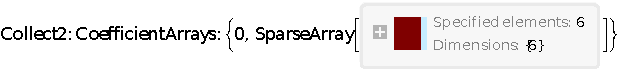
\includegraphics[width=0.6\linewidth]{img/1fqy7jqjvvk1u.pdf}
\end{figure}

\begin{dmath*}\breakingcomma
\text{Collect2: Collecting the monomials.}
\end{dmath*}

\begin{dmath*}\breakingcomma
\text{Collect2: tvm: }\left\{x,x^2,x^3,x^4,x^5,x^6\right\}
\end{dmath*}

\begin{dmath*}\breakingcomma
\text{Collect2: Done collecting the monomials, timing: }0.001726
\end{dmath*}

\begin{figure}[!ht]
\centering
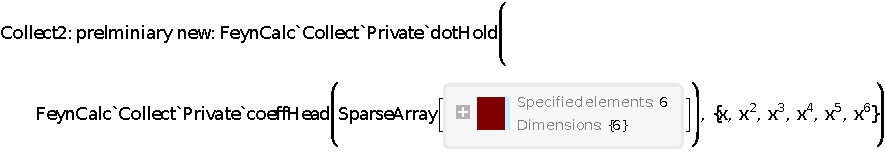
\includegraphics[width=0.6\linewidth]{img/0gyiguncykrsk.pdf}
\end{figure}

\begin{dmath*}\breakingcomma
\text{Collect2: Obtaining the final result.}
\end{dmath*}

\begin{dmath*}\breakingcomma
\text{Collect2: The final result is ready, timing: }0.001661
\end{dmath*}

\begin{dmath*}\breakingcomma
\text{Collect2: new: }\;\text{FeynCalc$\grave{ }$Collect$\grave{ }$Private$\grave{ }$unity} x^6-6 \;\text{FeynCalc$\grave{ }$Collect$\grave{ }$Private$\grave{ }$unity} (y+z) x^5+15 \;\text{FeynCalc$\grave{ }$Collect$\grave{ }$Private$\grave{ }$unity} (y+z)^2 x^4-20 \;\text{FeynCalc$\grave{ }$Collect$\grave{ }$Private$\grave{ }$unity} (y+z)^3 x^3+15 \;\text{FeynCalc$\grave{ }$Collect$\grave{ }$Private$\grave{ }$unity} (y+z)^4 x^2-6 \;\text{FeynCalc$\grave{ }$Collect$\grave{ }$Private$\grave{ }$unity} (y+z)^5 x
\end{dmath*}

\begin{dmath*}\breakingcomma
\text{Collect2: Releasing tempIso.}
\end{dmath*}

\begin{dmath*}\breakingcomma
\text{Collect2: Done releasing tempIso, timing: }0.000271
\end{dmath*}

\begin{dmath*}\breakingcomma
\text{Collect2: Putting re togehter.}
\end{dmath*}

\begin{dmath*}\breakingcomma
\text{Collect2: Done putting re togehter, timing: }0.000250
\end{dmath*}

\begin{dmath*}\breakingcomma
\text{Collect2: Done releasing tempIso, timing: }0.000510
\end{dmath*}

\begin{dmath*}\breakingcomma
\text{Collect2: Leaving.}
\end{dmath*}

\begin{dmath*}\breakingcomma
\text{Collect2: Leaving with}x^6-6 (y+z) x^5+15 (y+z)^2 x^4-20 (y+z)^3 x^3+15 (y+z)^4 x^2-6 (y+z)^5 x+(y+z)^6
\end{dmath*}

\begin{Shaded}
\begin{Highlighting}[]
\NormalTok{$VeryVerbose }\ExtensionTok{=} \DecValTok{0}\NormalTok{;}
\end{Highlighting}
\end{Shaded}

\end{document}
